\documentclass{article}
\usepackage{caption}
\usepackage{amssymb}
%\usepackage{array}
\usepackage{geometry}
%\usepackage{scrextend}
\usepackage{amsmath}
%\usepackage{hyperref}
\usepackage{graphicx}
\usepackage{pdfpages}
%\usepackage{multicol}
\usepackage{tabularx}
\usepackage{float}

\title{EE102 Homework 2}
\author{Jacob Guenther}

\geometry{
	a4paper,
	total={170mm,257mm},
	left=20mm,
	top=20mm,
}

\begin{document}

\includepdf[pages=1,pagecommand={}]{Lab_4_cover.pdf}

\section{Objective}

\section{Equipment}
\begin{itemize}
	\item Arduino Nano
	\item Resistor
	\item Thermistor
	\item LED
	\item Breadboard
	\item Jumpers
\end{itemize}

\section{Setup}
We use a voltage divider as seen in figure (1).

\begin{figure}[H]
	\begin{center}
	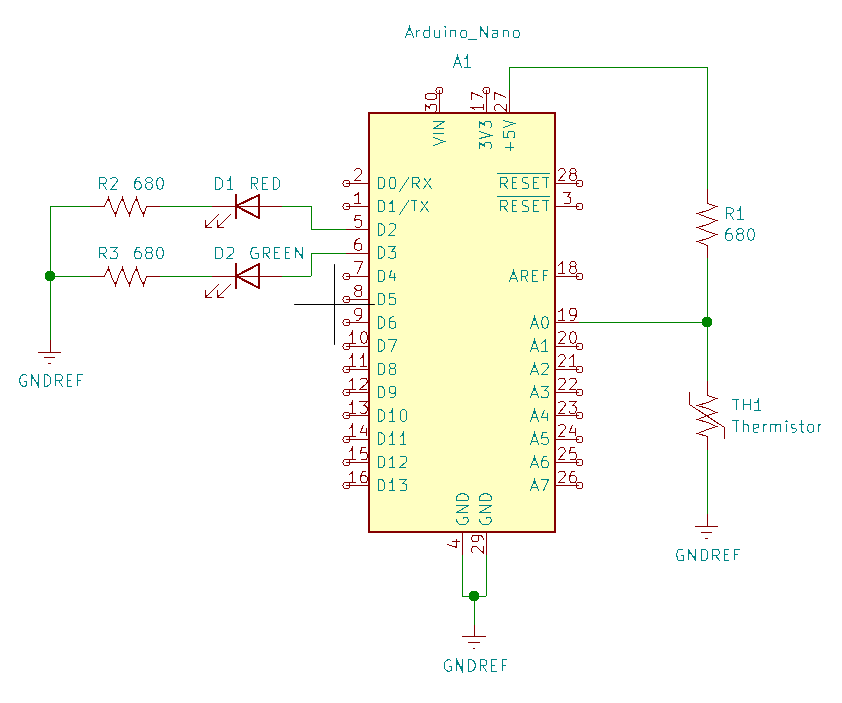
\includegraphics[width=10cm]{schematic}
	\end{center}
	\caption{Voltage divider using the thermistor connected to analog input 0.}
\end{figure}

\section{Observations and Results}

\paragraph{}

\paragraph{}

\begin{figure}[H]
	%\includegraphics[width=10cm]{code}
	\caption{Code used in this lab. Converts analog value to temperature.}
\end{figure}


\begin{table}[H]
\begin{tabular}{ | c | c | c | c | c | }
	\hline
	\textbf{Analog Input} &
	\textbf{Voltage} &
	\textbf{Temp Kelvin} &
	\textbf{Temp Celsius} &
	\textbf{Temp Fahrenheit} \\
	& (V) & (K) & (C) & (F) \\
	\hline
	963 & 4.52 & 296.27 & 23.12 & 73.61 \\
	\hline
	957 & 4.49 & 298.46 & 25.31 & 77.55 \\
	\hline
	953 & 4.47 & 299.83 & 26.68 & 80.03 \\
	\hline
	948 & 4.45 & 301.47 & 28.32 & 82.97 \\
	\hline
	947 & 4.44 & 301.79 & 28.64 & 83.54 \\
	\hline
	945 & 4.43 & 302.41 & 29.26 & 84.67 \\
	\hline
	943 & 4.42 & 303.02 & 29.87 & 85.77 \\
	\hline
	939 & 4.41 & 304.22 & 31.07 & 87.92 \\
	\hline
	937 & 4.40 & 304.80 & 31.65 & 88.97 \\
	\hline
	935 & 4.39 & 305.37 & 32.22 & 89.99 \\
	\hline
\end{tabular}
\caption{\label{tab:table-name} Voltages and temperatures logged at unique sensor reading values.}
\end{table}

\begin{figure}[H]
	%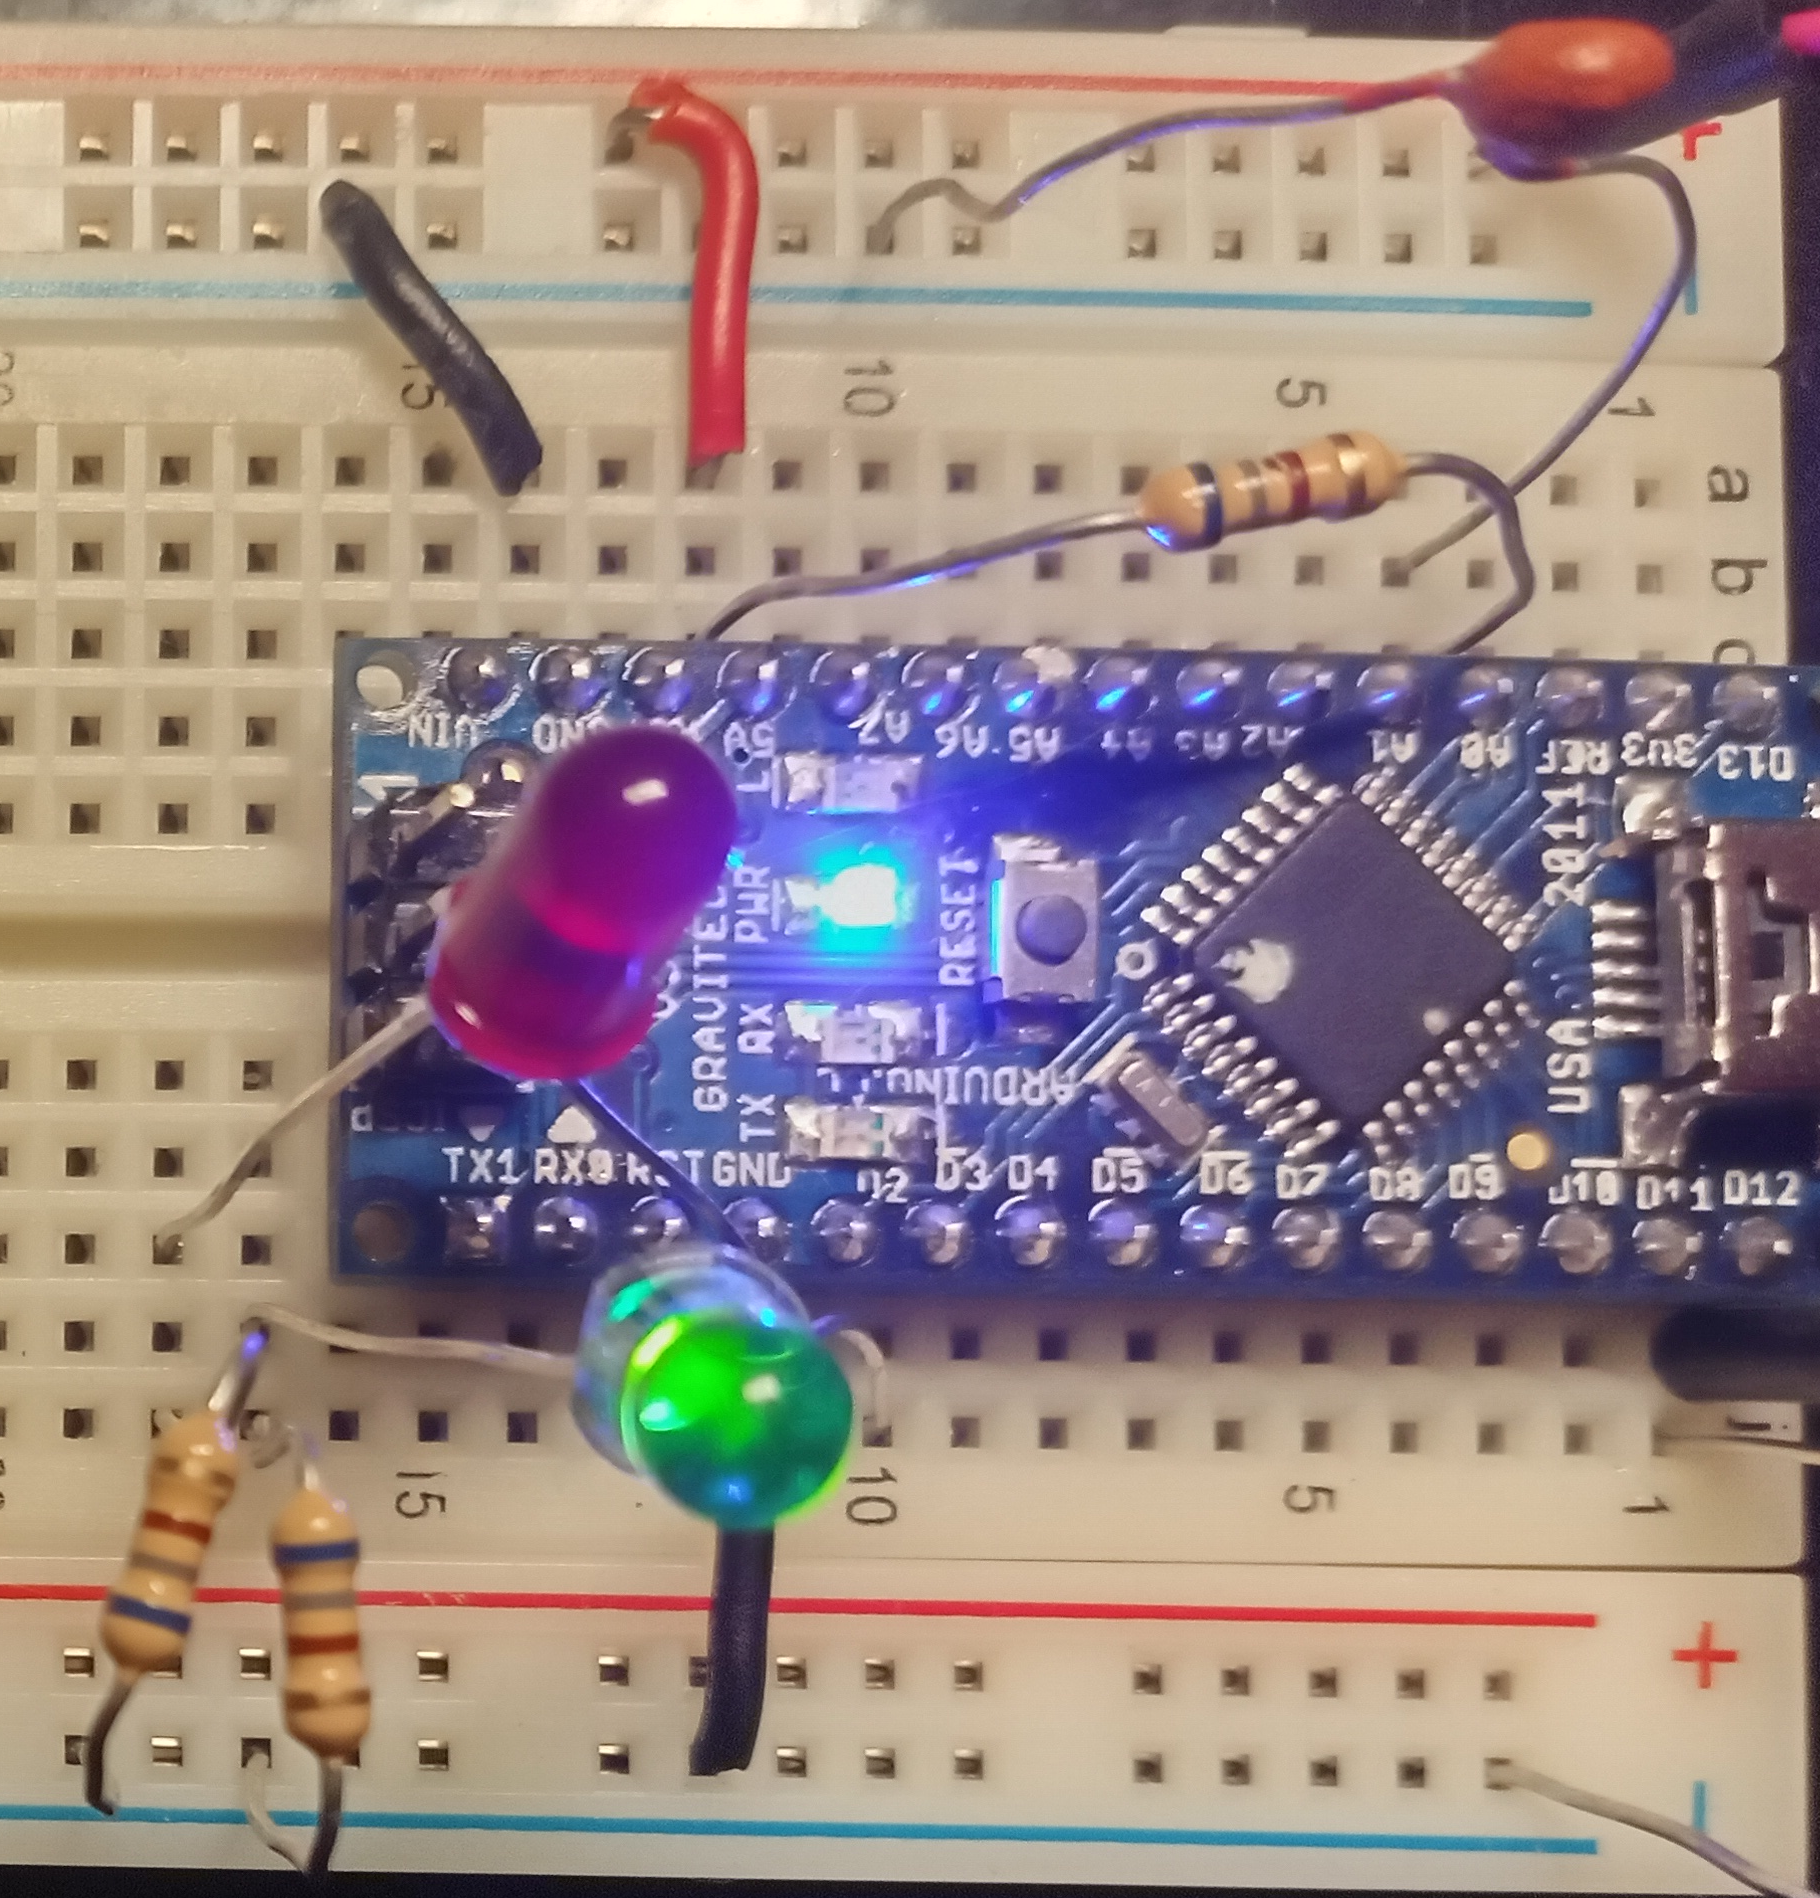
\includegraphics[width=10cm]{temp_below}
	\caption{Temperature below Celsius.}
\end{figure}

\begin{figure}[H]
	%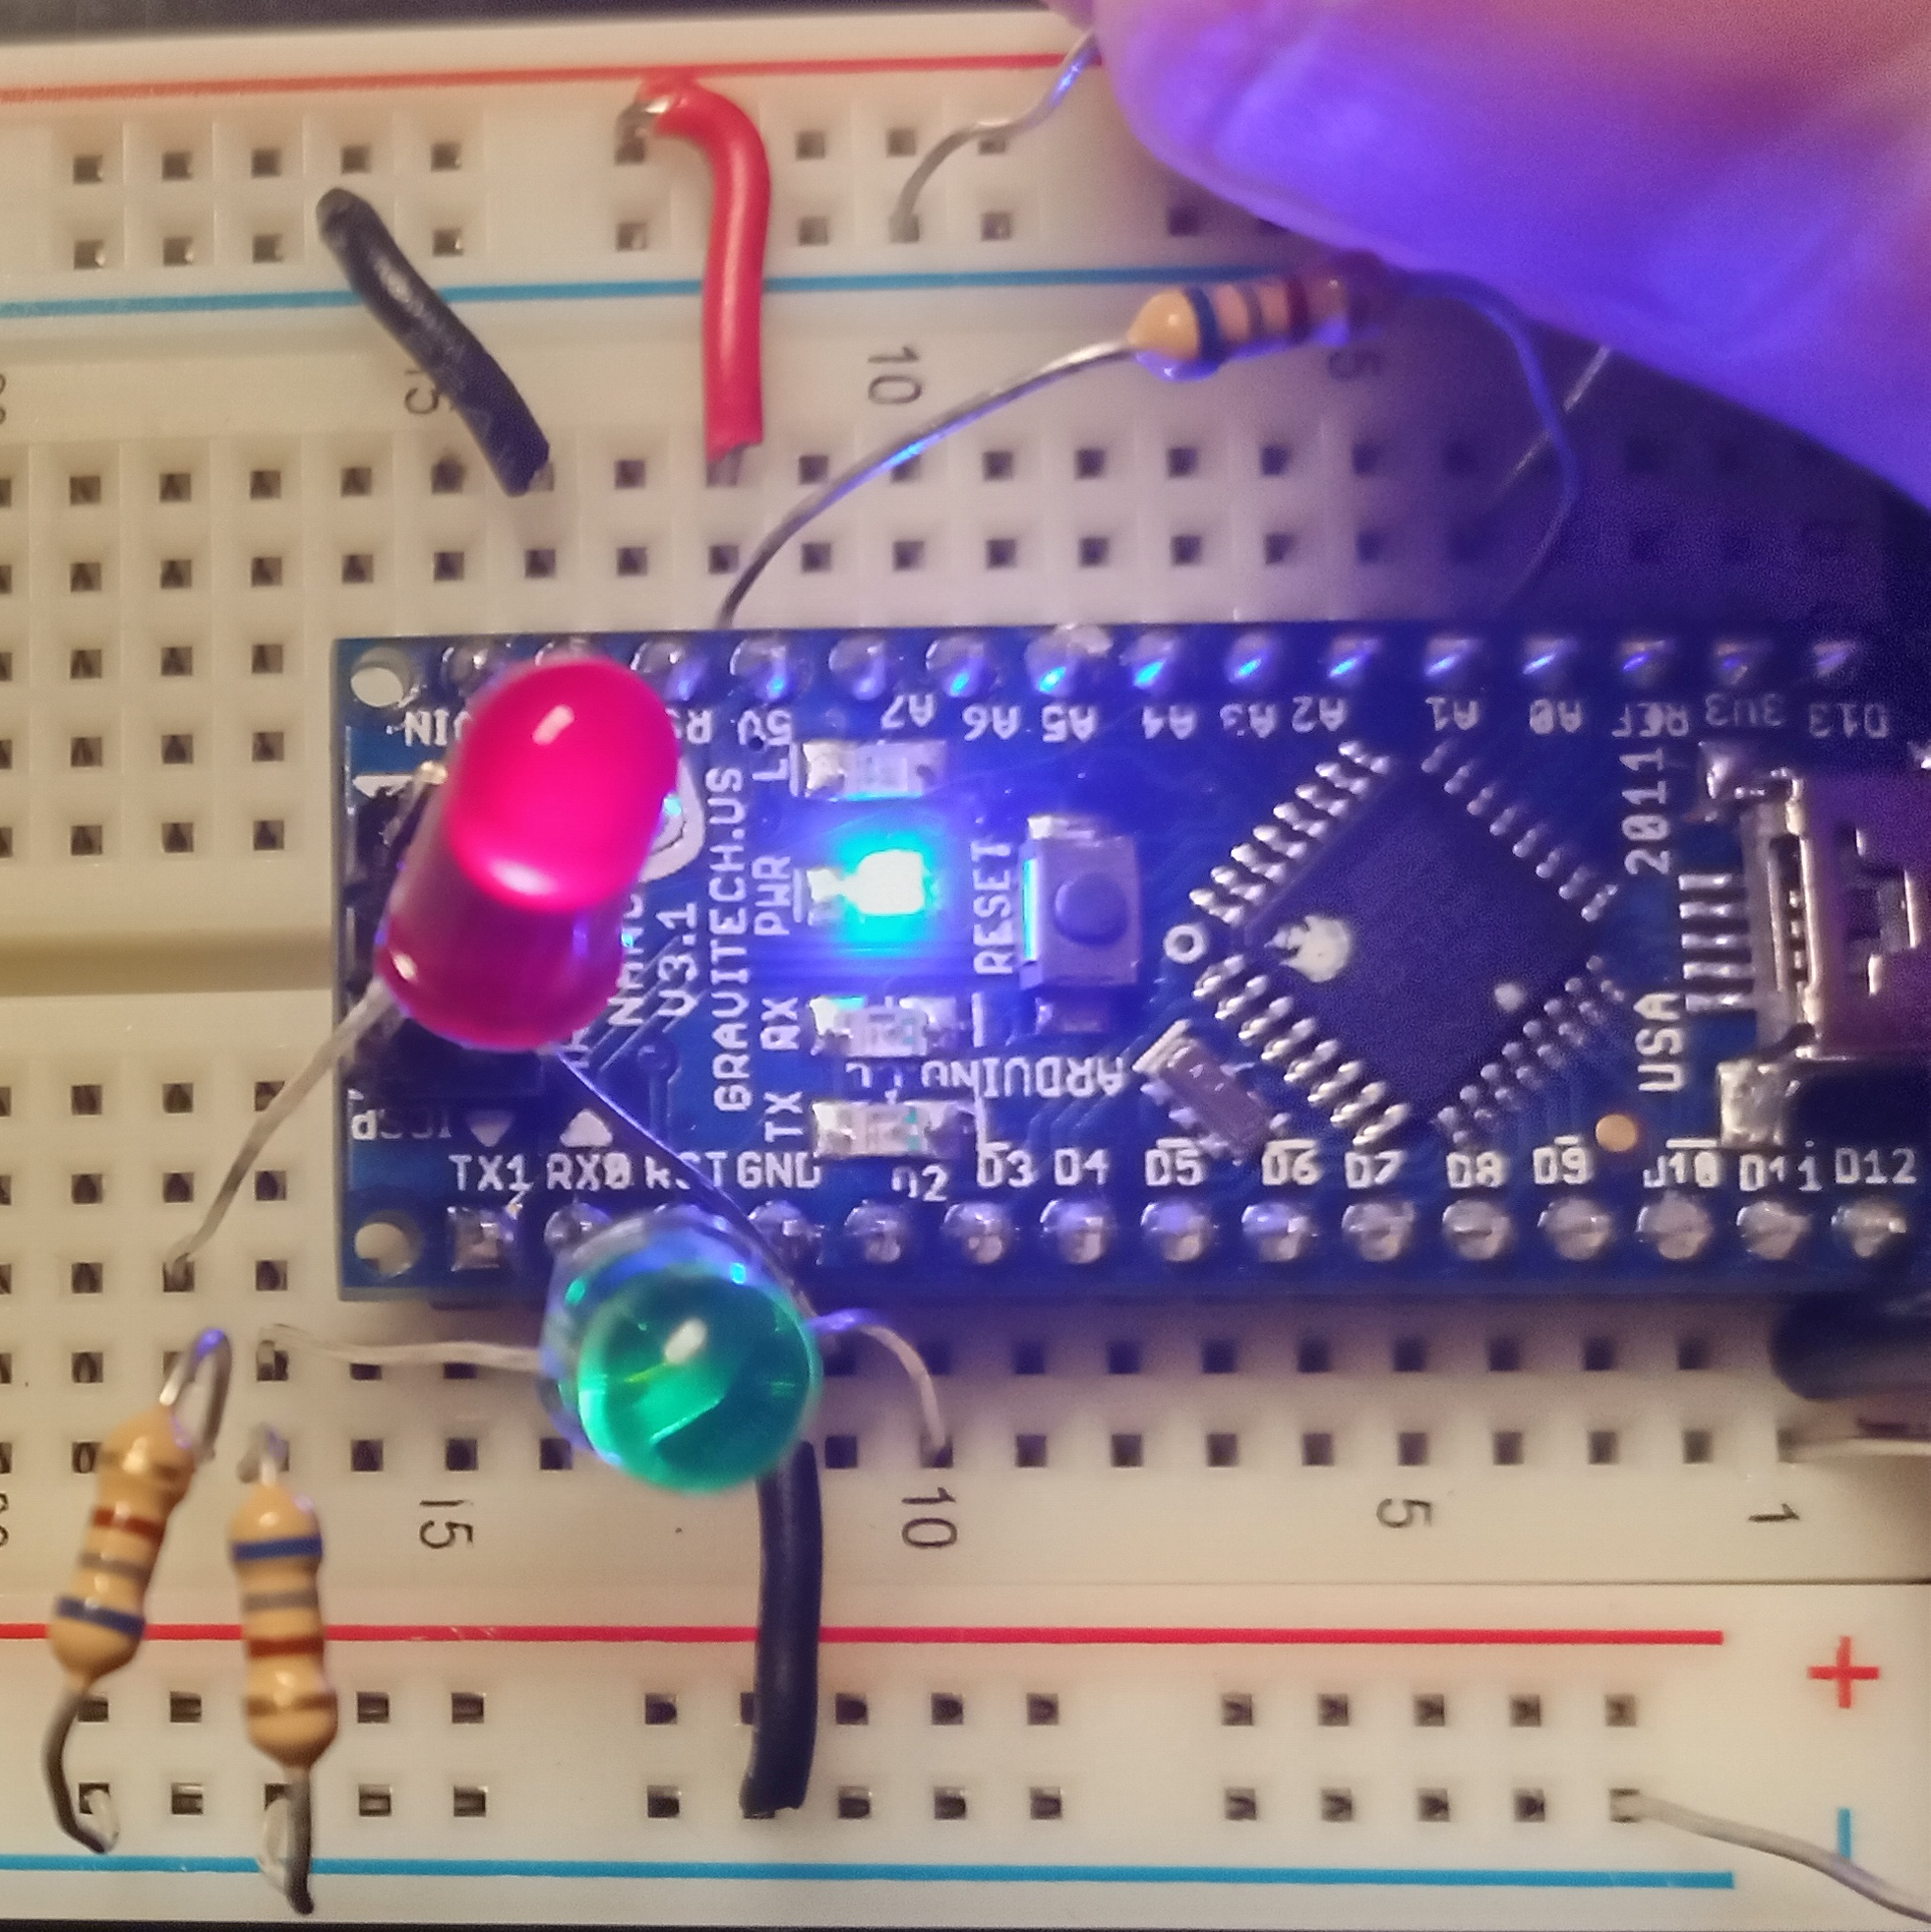
\includegraphics[width=10cm]{temp_above}
	\caption{Temperature above Celsius.}
\end{figure}

\newpage
\section{Conclusion}

\newpage
\section{References}
\noindent
[1] Denise Thorsen, Maher Al-Badri, INTRODUCTION TO ELECTRICAL AND COMPUTER ENGINEERING, University of Alaska Fairbanks, 2022.
\newline
\newline
\noindent

\end{document}